
%(BEGIN_QUESTION)
% Copyright 2006, Tony R. Kuphaldt, released under the Creative Commons Attribution License (v 1.0)
% This means you may do almost anything with this work of mine, so long as you give me proper credit

Beregn utgangsspenningen i denne op-amp-kretsen når inngangsspenningen minker (går i negativ retning) jevnt med -6.5 volt per sekund:

$$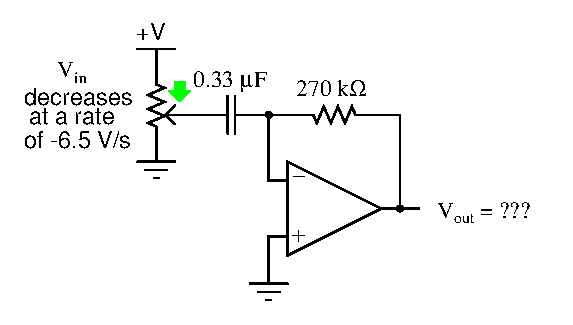
\includegraphics[width=15.5cm]{i01524x01.eps}$$

Beregn deretter ``tidskonstanten'' til denne deriveringskretsen (dvs. faktoren som relaterer utgangsspenning til inngangens endringsrate).

\underbar{file i01524}
%(END_QUESTION)





%(BEGIN_ANSWER)

$U_{ut}$ = 0.5792 volt

\vskip 10pt

$\tau_d$ = $RC$ = 89.1 ms

%(END_ANSWER)





%(BEGIN_NOTES)

Siden negativ tilbakekobling fra op-ampens utgang holder kondensatorens høyre terminal på jordpotensial, blir inngangsspenningen som faller med -6.5 V/s lagt direkte over kondensatoren. Vi vet at strømmen gjennom en kondensator beskrives av denne ligningen:

$$i_C = C{dv_C \over dt}$$
 

$$i_C = (0.33 \> \mu \hbox{F})(-6.5 \hbox{ V/s})$$
 

$$i_C = -2.145 \> \mu \hbox{A}$$
 
Denne lille strømmen, gjennom motstanden på 270 k$\Omega$, gir et spenningsfall på:

$$U = IR$$

$$U = (2.145 \> \mu \hbox{A})(270 \hbox{ k}\Omega)$$

$$U = 0.5792 \hbox{ volt}$$
 
Siden strømretningen (konvensjonell strømretning) er fra høyre mot venstre, blir dette spenningsfallet over motstanden positivt på høyre side og negativt på venstre side. Når venstre terminal av motstanden også er på jordpotensial (0 volt), blir utgangsspenningen {\it positiv} 0.5792 volt.
 
\vskip 10pt

Begrepet tidskonstant kan være enklere å forstå sett fra perspektivet til {\it enhetsanalyse}. Hvis inngangens endringsrate måles i enheten {\it volt per sekund}, og utgangen (som er proporsjonal med inngangens endringsrate) måles i enheten {\it volt}, må proporsjonalitetskonstanten måles i enheten {\it sekunder}:

$$\hbox{Ut} = k \hbox{ Inn}$$

$$\hbox{[V]} = k \left({\hbox{[V]} \over \hbox{[s]}}\right)$$

$$\hbox{[V]} = \hbox{[s]} \left({\hbox{[V]} \over \hbox{[s]}}\right)$$

$k$ må uttrykkes i tidsenheter (sekundet).

%INDEX% Electronics review: differentiator circuit

%(END_NOTES)
